%%%%%%%%%%%%%%%%%%%%%%%%%%%%%%%%%%%%%%%%%%%%%%%%%
% Relatório Final - Projeto de Pesquisa
% Métodos de Otimização
% Baltz & Machado
% Capítulo 1
%%%%%%%%%%%%%%%%%%%%%%%%%%%%%%%%%%%%%%%%%%%%%%%%%


\chapter{\Large{Métodos Matemáticos de Otimização}}\label{chp:1}


\section{{O Conceito de Otimização}}

\hspace{0.8cm}
Diz-se otimização, o processo que tem como objetivo encontrar condições que
minimizam ou maximizam algo (seja energia, tempo, dinheiro, etc). Sendo este,
muitas vezes um trabalho árduo, custoso.

Dessa maneira, na matemática, este processo é amplamente utilizado quando
busca-se valores pertencentes ao conjunto \textit{A} (que pode ter
restrições), com o objetivo de encontrar uma solução ótima, aplicando os valores
de \textit{A} em numa função objetivo predefinida.

Podendo assim, serem representadas da seguinte forma:

	Dada a função
	\begin{equation}
		f : A \rightarrow \mathbb{Z}
	\end{equation}

	\begin{itemize}
		\item Maximização pode ser definida como:
	\end{itemize}

		% TODO: Porque 'que satisfaz' está ficando errado?
		busca pelo elemento \textit{x_0} \in \textit{A}, que satisfaz:

			\begin{equation}
				f(x_0) \geq f(x);
			\end{equation}

		para todo x \in \textit{A}.\\


	\begin{itemize}
		\item Minimização pode ser definida como:
	\end{itemize}

		% TODO: Porque 'que satisfaz' está ficando errado?
		busca pelo elemento \textit{x_0} \in \textit{A}, que satisfaz:

			\begin{equation}
				f(x_0) \leq f(x);
			\end{equation}

		para todo x \in \textit{A}.\\


Com isso, podemos agora entender como esse processo pode ser custoso.
Começando pelo fato de que existem os pontos máximos e mínimos
(pontos críticos), locais e globais no espaço das funções. Sendo os pontos
críticos locais, aqueles que não são os menores ou maiores valores para a
minimização e maximização, respectivamente. E os pontos globais, aqueles que
representam o menor ou maior valor no espaço da função, para a minimização e
maximização, respectivamente.

Criando assim, uma certa incerteza ao encontrar um valor crítico numa função,
já que é estritamente difícil saber se o ponto crítico encontrado é local ou
global.Como pode-se perceber na Figura
\ref{grafico_local_global_pontosCriticos}.


\begin{figure}[h]
	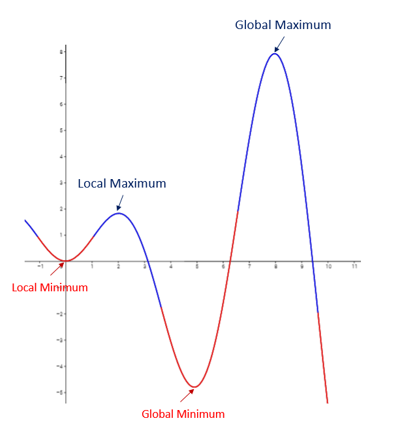
\includegraphics[width=0.43\textwidth]
	{src/grafico_local_global_pontosCriticos.png}
	\centering
	\caption{Exemplo de pontos críticos locais e globais indicados no gráfico
	de uma função}
	\label{grafico_local_global_pontosCriticos}
\end{figure}




\section{{Otimização de Funções à Uma variável real}}

\hspace{0.8cm}






\section{{Programando o Método}}

\hspace{0.8cm}





\textcolor[rgb]{1,0,0}{\section{{Otimização de Funções à Várias Variáveis}}}

\hspace{0.8cm}





%
